\chapter{Experimental}

\section{P3HT Batch Synthesis}

\subsection{Synthesis}

4 g of 1,2-dibromomethane was added to a two-neck round-bottomed flask and degassed under vacuum for 10 minutes. Argon gas was then introduced to the flask to provide an inert atmosphere. 40 ml of THF was injected into the system, followed by 6 mL of 1M isopropyl magnesium chloride. The flask was stirred and heated at 55 C for 1 hour to produce the active thiophenyl Grignard reagent. Nickel II bromide (diphenylphosphnoprane) complex (Ni(dppp)Br2) was then added to the reaction, and left to stir at 55 C for a further hour for polymerisation to occur. The reaction was cooled, and 50 ml of methanol was added to quench the reaction and cause the precipitation of P3HT out of solution. The resultant slurry was filtered under gravity and washed with acetone.

\subsection{Purification}

The crude wet P3HT was purified in a Soxhlet extractor using a solvent mix of equal parts n‑hexane, ethyl acetate and acetone. This solvent mixture extracted impurities from the solid, leaving a purer product in the cellulose thimble. The extraction process was run for 24 hours. The thimble was then moved to a clean Soxhlet extractor using chloroform as an extraction solvent. The extraction process was run for a further 24 hours. The chloroform solution was cooled, concentrated on a rotary evaporator, and methanol was added to induce precipitation of the P3HT. The solution was then placed on a rotary evaporator until all the solvent had been removed, yielding pure P3HT.


\section{P3HT Droplet Flow Synthesis}

\subsection{Reagent Preparation}

2 - 4 g of 1,2-dibromomethane was added to a two-necked round-bottomed flask and degassed under vacuum for 10 minutes. Argon gas was then introduced to the flask to provide an inert atmosphere. 20 - 40 ml of THF was injected into the system, followed by 3 -6 mL of 1M isopropyl magnesium chloride. The flask was stirred and heated at 55 C for 1 hour to produce the active thiophenyl Grignard reagent.

In a second two-necked round-bottomed flask, Nickel(II) bromide ethylene glycol dimethyl ether complex (Ni(dme)Br2) and 1,3-bis(diphenylphosphino) propane were added and placed under an inert Argon atmosphere. 40 ml of THF was injected to form a pale pink solution, and left to stir for an hour.

In a third two-necked round-bottomed flask, Nickel(II) bromide ethylene glycol dimethyl ether complex and triphenylphosphine were added and placed under an inert Argon atmosphere. 40 ml of THF was injected to form a green solution, and left to stir for an hour to form Nickel (II) Bromide bis-triphenylphosphino complex.

\subsection{Synthesis}

Syringe pumps were used to produce continuous streams of the active thiophenyl Grignard reagent in THF, the Ni(dppp)Br2 in THF, and the perfluorinated polyether Galden. The three streams were mixed in a flow mixer to form a stream of THF droplets in Galden. The droplet stream was then passed through an oil bath at 55 C with a residence time of five minutes to induce polymerisation. The droplet stream was then passed through a second mixer with a stream of the Ni(TPP)2(Br2) solution to terminate any remaining Grignard reagent. The two-phase droplet stream was then passed into a liquid-liquid separator to separate out the Galden and THF phases. The outlet THF stream containing the P3HT product was periodically analysed by an inline GPC column, and then collected in acidified methanol to induce precipitation.

\section{Analysis}

Off-line analysis of P3HT molecular weight and polydispersity was performed on an Agilent Gel Permeation Chromatography instrument, calibrated with polystyrene standards. 

\section{Programming}

Control of the in-line GPC system was coded in LabVIEW software, consisting of a “front panel” which acts as a control board for the program, and a “block diagram” where the code is written. A flow diagram showing the operation of the GPC system can be seen in Figure 14. 

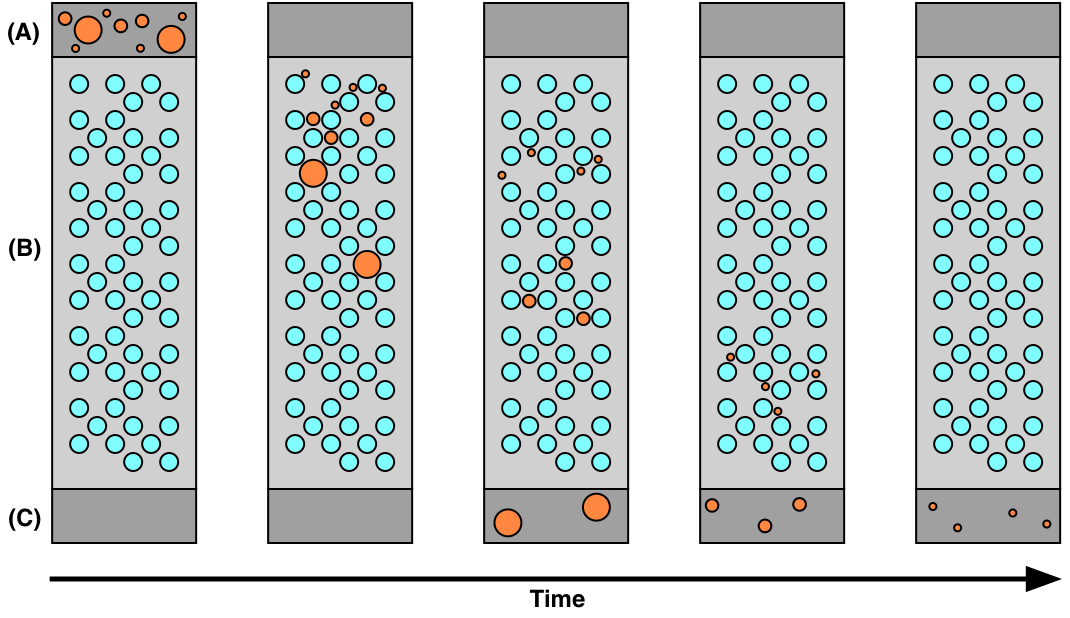
\includegraphics{GPC_Operation}

The analysis and flow monitoring at the separator was initially coded in Arduino and MATLAB. The Arduino code read the analog output from the photodiode every X seconds. The data was transferred to MATLAB where it was plotted in real time. 

